\documentclass[11pt]{article}
\usepackage[letterpaper,margin=1in]{geometry}
\usepackage[T1]{fontenc}
\usepackage{lmodern,microtype,amsmath,amssymb,amsthm,xcolor,tcolorbox}
\tcbuselibrary{skins}
\usepackage{graphicx}
\usepackage[hidelinks]{hyperref}
\definecolor{routegreen}{HTML}{128675}
\definecolor{ink}{HTML}{213337}
\newtcolorbox{takeaway}{enhanced,colback=routegreen!5!white,
 colframe=routegreen!5!white,colupper=ink,boxrule=0pt,
 borderline west={2pt}{0pt}{routegreen},arc=2mm,boxsep=0pt,
 left=3mm,right=3mm,top=1.5mm,bottom=1.5mm,
 before skip=5pt,after skip=5pt,fontupper=\sffamily\small}
\newtcolorbox{algorithm}{colback=ink!3!white,colframe=ink,
 colbacktitle=ink,coltitle=white,title=Construction: longest admissible group,
 fonttitle=\sffamily\small\bfseries,fontupper=\ttfamily\small,
 boxrule=.4pt,arc=2mm,left=3mm,right=3mm,top=2mm,bottom=2mm}
\newtheorem{theorem}{Theorem}
\newtheorem{corollary}[theorem]{Corollary}
\setlength{\parskip}{3pt}
\setlength{\parindent}{0pt}
\begin{document}
\begin{center}
{\LARGE Compressing Road Chains Under a\\[2pt] Variable Edge-Cost Floor}\par\vspace{5pt}
{\large Jonathan R. Landers}\par
November 22, 2026
\end{center}

\section*{1. A shortcut that works for many floors}
Consider repeated shortest-path queries in a weighted graph. Each query
sets a minimum charge for traversing an edge. Our goal is to compress
chains of edges while bounding the resulting error for every such charge.
Road networks provide one interpretation: vertices are junctions or points
along a road, and edge costs represent distance or travel time.

Formally, let the network be a finite undirected graph
\[
 G=(V,E),\qquad w:E\to[0,\infty),
\]
where $V$ is the set of vertices, $E$ is the set of edges, and $w(e)$ is
the finite cost of traversing edge $e$. A route's cost is the sum of its
edge costs. A query chooses a floor $k\ge0$, giving each edge the charge
\[
 w_k(e)=\max\{w(e),k\}.
\]
A chain is a path whose internal vertices have degree two, meaning each
has exactly two incident edges. Replacing it by a shortcut edge between
its endpoints removes intermediate routing decisions. The shortcut's charge must reflect the floor on each original
edge: two edges of cost one have total charge six at floor three, whereas
flooring their original sum gives three.

We group similar edge costs and represent each group by its mean. We derive
exact error formulas, build the smallest summary for a chosen tolerance,
and use shortcut errors to certify the quality of a returned route.

\paragraph{The exact cost and its summary.}
Let a chain contain $h\ge1$ finite, nonnegative edge costs. Sort them:
\[
 0\le w_1\le w_2\le\cdots\le w_h.
\]
Sorting serves only to build the cost summary. Retain the original road
order separately so that a shortcut can later be expanded into a route.
Divide the sorted indices into $r$ nonempty consecutive groups: each group
is a block of adjacent entries in this order. For group
$G_j$, store its number of edges and its mean cost:
\[
 h_j=|G_j|,\qquad \mu_j=\frac{1}{h_j}\sum_{i\in G_j}w_i.
\]
The exact chain cost and the summary cost at floor $k\ge0$ are
\begin{equation}\label{cost}
 \begin{aligned}
 C(k)&=\sum_{i=1}^h\max(w_i,k),\\
 \widehat C(k)&=\sum_{j=1}^r h_j\max(\mu_j,k).
 \end{aligned}
\end{equation}
For costs $(1,3)$, one group stores size two and mean two. At floor two,
the exact cost is five and the summary gives four.

\newpage
\section*{2. What determines the error?}
Two measures of spread within each group will describe the error:
\[
 A_j=\frac12\sum_{i\in G_j}|w_i-\mu_j|,\qquad
 V_j=\sum_{i\in G_j}(w_i-\mu_j)^2.
\]
The first measures absolute deviations from the mean; the second measures
squared deviations. They answer two different questions: how large can the
error become, and what is its average when floors are sampled uniformly?

\begin{theorem}[Exact compression errors]\label{thm:error}
For every nonnegative floor, the summary underestimates the chain cost.
Its largest error across all floors is exactly
\begin{equation}\label{uniform}
 0\le C(k)-\widehat C(k),\qquad
 \sup_{k\ge0}\bigl(C(k)-\widehat C(k)\bigr)=\max_j A_j.
\end{equation}
If the query floor is a random variable $K$ uniform on $[0,U]$, with
$U>0$ and $w_h\le U$, its expected error is
\begin{equation}\label{average}
 \mathbb E\bigl[C(K)-\widehat C(K)\bigr]=\frac{1}{2U}\sum_j V_j.
\end{equation}
\end{theorem}
\begin{takeaway}
The worst group determines the largest error across all floors; squared
spread within groups determines average error under a uniform floor.
\end{takeaway}
\begin{proof}
Consider one group $G$ of size $q$ and mean $\mu$. Its error is
\[
 g_G(k)=\sum_{i\in G}\max(w_i,k)-q\max(\mu,k).
\]
The function $w\mapsto\max(w,k)$ is convex, so replacing the costs by their
mean can only decrease their total charge. Thus $g_G(k)\ge0$.
For floors below $\mu$, the summary is constant while the exact cost is
nondecreasing. Above $\mu$, the summary has slope $q$, while the exact
cost has slope at most $q$. The error therefore peaks at $\mu$, where
\[
 g_G(\mu)=\sum_{i\in G}(w_i-\mu)_+
 =\frac12\sum_{i\in G}|w_i-\mu|.
\]
Here $(x)_+=\max(x,0)$; deviations above and below the mean have equal total.
The error is zero whenever the floor lies outside the group's cost range,
including its endpoints. Consecutive groups in sorted order have disjoint
range interiors. Consequently, at most one group contributes error at any
floor. This proves \eqref{uniform}.

This also explains why group errors do not add: a group introduces error
only while the floor passes through its own interval of costs. Errors
from separate shortcuts along a route can occur at the same floor; these
will add in the route certificate below.
\end{proof}

\paragraph{How the floor changes cost.}
Away from an original cost, each edge below the floor contributes one
to the slope of the exact charge. A group whose mean is below the floor
contributes its size to the summary's slope:
\[
 C'(k)=|\{i:w_i<k\}|,\qquad
 \widehat C'(k)=\sum_{j:\mu_j<k}h_j.
\]
The summary replaces several smaller slope changes by one larger change
at each group mean. The next page shows the resulting gap and completes
the average-error proof.

\newpage
\section*{3. A worked example and its average error}
Take four costs, divided into two groups of sorted indices:
\[
 (w_1,w_2,w_3,w_4)=(1,3,6,10),\qquad
 G_1=\{1,2\},\quad G_2=\{3,4\}.
\]
Both groups have size two; their means are two and eight. Thus
\[
 \begin{aligned}
 C(k)&=\max(1,k)+\max(3,k)+\max(6,k)+\max(10,k),\\
 \widehat C(k)&=2\max(2,k)+2\max(8,k).
 \end{aligned}
\]
The group errors are $A_1=1$ and $A_2=2$, so the largest chain error is
two. At floor eight, the exact charge is $34$ and the summary gives $32$.

\begin{center}
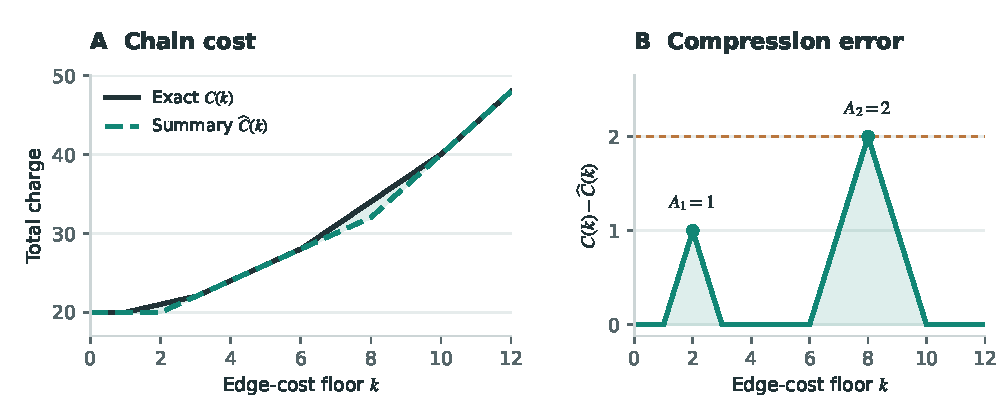
\includegraphics[width=\linewidth]{figures/floor_response.pdf}\par
\small\textbf{Figure 1.} Exact and summary charges change slope at the
original costs and group means, respectively. The shaded error occurs
within each group's cost range. Peaks occur at means $2$ and $8$;
the larger peak gives the uniform error certificate.
\end{center}

\paragraph{Completing the average-error proof.}
For a uniform floor on $[0,U]$, expected error is the area under the
error curve divided by $U$. Split each charge's integral at its cost:
\[
 \int_0^U\max(w,k)\,dk
 =\int_0^w w\,dk+\int_w^U k\,dk
 =w^2+\frac{U^2-w^2}{2}=\frac{U^2+w^2}{2}.
\]
This holds for $0\le w\le U$, including every group mean. Since group
sizes sum to $h$, subtracting the summary integrals cancels the $U^2$
terms. Hence
\[
 \begin{aligned}
 \int_0^U(C(k)-\widehat C(k))\,dk
 &=\frac12\sum_j\left(\sum_{i\in G_j}w_i^2-h_j\mu_j^2\right)\\
 &=\frac12\sum_j\sum_{i\in G_j}(w_i-\mu_j)^2.
 \end{aligned}
\]
Expanding the squares gives the last equality because
$\sum_{i\in G_j}w_i=h_j\mu_j$. Division by $U$ proves \eqref{average}.
In the example, with $U=12$, the squared deviations sum to $2+8=10$,
so expected error is $5/12$.

\newpage
\section*{4. Build the smallest summary for a tolerance}
Choose an allowed error $\varepsilon\ge0$. Theorem~\ref{thm:error} turns a
condition on every possible floor into a simple test on each group:
\[
 \sup_{k\ge0}(C(k)-\widehat C(k))\le\varepsilon
 \quad\Longleftrightarrow\quad A_j\le\varepsilon\text{ for every group }j.
\]
This lets us grow each group until adding the next cost would break the bound.

\begin{theorem}[Fewest groups at a prescribed tolerance]\label{thm:greedy}
Repeatedly taking the longest next group with error at most $\varepsilon$
uses the fewest groups among all consecutive partitions represented by
sizes and means that meet the uniform tolerance. Construction takes
\[
 O(h\log(h+1))\text{ time},\qquad O(h)\text{ working space}.
\]
\end{theorem}
\begin{takeaway}
For a chosen worst-case error, the greedy rule stores the fewest groups
within this family of summaries.
\end{takeaway}
\begin{algorithm}
01 Sort the costs and build prefix sums.\par
02 Start a group with the next unassigned cost.\par
03 While the next cost keeps group error <= epsilon:\par
\hspace*{5mm}append that cost to the group.\par
04 Store the group's (size, mean).\par
05 Repeat from 02 until every cost is assigned.\par
06 Store cumulative group counts and weighted means.
\end{algorithm}
\begin{proof}
Use $g_B(k)$ for the group error defined in the previous proof, with the
mean recomputed for group $B$. First observe that removing entries cannot increase its
maximum error. To see this, split a group into disjoint nonempty parts
$B$ and $D$. Convexity applied to their two means gives
\[
 g_{B\cup D}(k)\ge g_B(k)+g_D(k)\ge g_B(k).
\]
Taking maxima proves the claim.

Now compare the greedy first group with any feasible partition. That
partition's first group must end no later than the greedy group, since
greedy takes the longest feasible prefix. Replace all entries covered by
the greedy group with that single group. If its endpoint falls inside an
existing group, keep the remaining suffix of that group. Removing entries
preserves feasibility, and this replacement uses no more groups. Repeating
on the remaining list transforms an optimal partition into the greedy
partition without increasing its size. This proves optimality.

For the running time, a prefix-sum array stores the sum of the first $i$
sorted costs at position $i$. Subtracting two entries gives any group's
sum, and hence its mean, in constant time.
Binary search finds the $q_-$ entries strictly below that mean. Their sum
gives its error as
\[
 A=q_-\mu-\sum_{\substack{i\in G\\w_i<\mu}}w_i.
\]
Each feasibility test takes $O(\log(h+1))$ time. Each cost is tested at
most twice: once as an extension, and possibly again as a new group.
Together with sorting, this proves the stated construction bounds.
\end{proof}

\newpage
\section*{5. Answer queries and certify routes}
\enlargethispage{\baselineskip}
\setlength{\abovedisplayskip}{7pt}
\setlength{\belowdisplayskip}{7pt}
\setlength{\parskip}{2pt}
The group means are sorted. For a query floor $k$, binary search finds
the last mean at most $k$. Let $\ell=0$ if none qualifies. Empty sums
are taken to be zero. Then
\[
 \widehat C(k)=k\sum_{j\le\ell}h_j+\sum_{j>\ell}h_j\mu_j.
\]
Cumulative counts and weighted means give the sums in constant time after
the search. Each shortcut needs
\[
 O(\log(r+1))\text{ time per query},\qquad O(r)\text{ summary space}.
\]
Retain road geometry and original edge order separately for reconstruction.

The average-error formula offers another design objective. With uniform
floors and a fixed number of groups, minimizing expected chain error is
equivalent to minimizing
\[
 \sum_j\sum_{i\in G_j}(w_i-\mu_j)^2.
\]
This is one-dimensional squared-error clustering for a fixed chain. A route
chosen after observing the floor also requires accounting for that choice.

\paragraph{From shortcut errors to route quality.}
Return to the graph $G=(V,E)$ from Section 1. Choose distinct terminals
$s,t$ (the query's start and destination) joined by a path. Replace chains whose internal vertices have degree two
by shortcuts. Keep $s,t$ as vertices and preserve parallel shortcuts, so
that distinct roads remain available. Assign each shortcut $e$ a summary
with uniform error bound $\varepsilon_e$. At any floor $k$, this means
\[
 0\le C_e(k)-\widehat C_e(k)\le\varepsilon_e.
\]
For a shortcut path $P$, write $C(P,k)$ and $\widehat C(P,k)$ for its total
exact and summary costs. Let $d(k)$ be the exact shortest $s$--$t$ distance
with original edges floored at $k$.

\begin{corollary}[Route certificate]
If $\widehat P$ minimizes summary cost, its expanded route satisfies
\[
 0\le C(\widehat P,k)-d(k)\le\sum_{e\in\widehat P}\varepsilon_e.
\]
\end{corollary}
\begin{takeaway}
Adding the shortcut certificates along the returned route bounds how
much more that route costs than an exact optimal route.
\end{takeaway}
\begin{proof}
Let $P^*$ be an exact optimal route, represented by its shortcuts.
Optimality under the summary costs and their lower-bound property give
\[
 \widehat C(\widehat P,k)\le\widehat C(P^*,k)\le C(P^*,k)=d(k).
\]
The selected route's exact cost is at most its summary cost plus the sum
of its shortcut errors. Combining these inequalities proves the bound.
\end{proof}

{\footnotesize
\textit{Related work.} Approximate shortcut functions are established in
routing~[1]. Positive-part expectations and their approximation are studied
through stop-loss transforms~[2]. The results here characterize error and
optimal consecutive grouping for the particular floor family \eqref{cost}.\par
[1] G. V. Batz, R. Geisberger, S. Neubauer, and P. Sanders.
\href{https://ae.iti.kit.edu/download/sea10_atch.pdf}{Time-Dependent
Contraction Hierarchies and Approximation}. SEA, 2010, pp.~166--177.\par
[2] W. H\"urlimann.
\href{https://www.kurims.kyoto-u.ac.jp/EMIS/journals/BAMV/conten/vol15/bamvXV-2.pdf}{Extremal
Moment Methods and Stochastic Orders}, Chapters IV--VI.
\textit{Bol. Asoc. Mat. Venezolana} 15(2), 2008.
}
\end{document}
